% Chapter 1

\chapter[Motivation and Background]
{Motivation and Background} % Main chapter title

\label{Chapter1} % For referencing the chapter elsewhere, use \ref{Chapter1} 

%----------------------------------------------------------------------------------------






% Define some commands to keep the formatting separated from the content 
\newcommand{\keyword}[1]{\textbf{#1}}
\newcommand{\tabhead}[1]{\textbf{#1}}
\newcommand{\code}[1]{\texttt{#1}}
\newcommand{\file}[1]{\texttt{\bfseries#1}}
\newcommand{\option}[1]{\texttt{\itshape#1}}

%----------------------------------------------------------------------------------------

\section[Quantum information processing and Qubit candidates]{Quantum information processing and Qubit candidates}

The bit is the basic unit of information in computing and digital communications. A bit can have one value, which can be 1 or 0, that represents the logical states in a 2-level logic system. In modern digital computers, these two states exits as low and high voltages in highly integrated circuits. Just like a bit for classical computing, a qubit is the basic unit of information in Quantum Information Processing (QIP), which encodes 1 and 0 into 2 distinguishable quantum states. As the qubits behave in the manner of quantum mechanism, it gives rise to the phonomena of superposition and entanglement, the computing power increases exponentially while more qubits adding up together. Previous difficult tasks in classical computing such as simulation of quantum systems or factoring of numbers would be finished quickly and efficiently by quantum computers.

For the realisation of a quantum computer,  the first priority is to find a suitable candidate as qubit. Five principles have been brought up for the candidates choosing by \citep{divincenzo_physical_2000}:

1. A scalable physical system with well characterized qubits

2. The ability to initialize the state of qubits to a simple fiducial state

3. Long relevant decoherence times, much longer than gate operation time

4. A "universal" set of quantum gates

5. A qubit-specific measurement capability

Color centres are optically active impurities that are responsible for the colors in crystals that are transparent due to large band gap. They are atom-like solid systems that, with appropriate electronic structure and symmetry in crystal, can be the candidates for qubits. Additionally, it is practical to require a long enough coherent time for information storage, thus quantum information processing can happen.  

Lots of research has been done with the negative charged nitrogen vacancy (NV$^{-}$), which has excellent spin properities at ambitent condition \citep{childress_atom-like_2014}, it has also been proved that it is possible to execute an all optical access to its spin. \citep{bassett_ultrafast_2014,buckley_spin-light_2010,santori_coherent_2006-1}. Yet due to the transform of symmetry during the excitation process, NV$^{-}$ has a big phonon side band following the zero-phonon line (ZPL). Moreover, the C$_{3v}$ symmetry leaves the color centre vulnerable towards the environment electric field, resulting in spectral diffusion, which is caused by the flipping of charging state. These disadvantages has reduced the generation rate of coherent photon generation rates and limit the development of NV-quantum networks \citep{rogers_all-optical_2014}.
%----------------------------------------------------------------------------------------

\section[Silicon vacancy as a Qubit candidate]{Silicon vacancy as a Qubit candidate}

Negative charged Silicon vacancy centres (SiV$^{-}$) are considered as the next promising qubit candidate after NV$^{-}$. It has irresistibly excellent optical properties, and is also possible to achieve an all optical intiallizaiton, read out and coherent preparation.

SiV$^{-}$ has a D$_{3d}$ symmetry with the symmetry axis along the <111> crystal direction. The color center consists of a substitial Silicon atom and a carbon vacancy. Due to the size difference between Silicon atoms and carbon atoms, it is expected that the Silicon atom will sit between 2 lattice site instead of on a lattice site\citep{goss_twelve-line_1996, gali_textitab_2013}. The inversion symmetry offers SiV$^{-}$ extra shielding from the small electric field fluctuation.

Experimentally it is observed that the SiV$^{-}$ has outstanding optical properties, 70$\%$ of its fluorescence coupled into a sharp ZPL at 1.68eV \cite{wang_single_2006}. At cryogenic temperature this ZPL can be resolved with a fine structure of 4 lines. These four lines correspond to the electronic transitions between the ground state and the first excited state of SiV$^{-}$. Theoretical calculation based on group theory and ab initio methods offer us a model of the SiV$^{-}$ electronic structure with a ground state of 2-fold degeneracy and even parity, a first excited state of 2-fold degeneracy of uneven parity and a second excited state of no degeneracy with even parity. \citep{goss_twelve-line_1996} This calculation fits the observation as only the electronic transition between levels of different parity is allowed, due to the -1 parity of photons, thus only the 4 transitions between the first excited state and the ground state would be allowed, corresponding to the 4 line structure of ZPL. Since this is a E to E transition, no dramatic symmetry change has been involved, less phonon would be involved in the relaxation, which fits the observation of the sharp ZPL with small phonon side band. 

Rogers et al. showed the probility to read out and coherently prepare electronic spin in individual SiV$^{-}$ centers via resonance excitation. As shown in the \ref{fig:CPT} The SiV$^{-}$ was first initialized by resonantly pumping the spin-flipping transition D1 that is weakly allowed due to the off axis residue of the magnetic field, this is done with applying a laser pulse that resonant to transition D1. After a dark interval the spin state was read out using a laser pulse on the cycling transition D2. The leading edge peak from D2 pulse will decrease with the increase of dark interval approaching an minimum. From this the spin relaxation time T1 has be calculated as 2.4 $\pm$ 0.2ms. With the similar pulse measurement, the orbital T1 has been measured as 38 $\pm$ 1ns. The fact that the orbital T1 is much shorter that spin T1 indicates that the orbital relaxation is highly spin conserving, indicates that this is a phonon transition.  The temperature dependency measurement reveals that the orbital rate increase linear with the temperature until 22K, which indicates a single-phonon mechanism of orbital relaxation.\citep{rogers_all-optical_2014,orbach_spin-lattice_1961,rogers_electronic_2014,scott_spin-lattice_1962}

Further coherent population trapping (CPT) was carried out by tuning the pump laser to transition D2 while scanning across the transition D1 using the probe laser. The spin coherence time was then measured to be 35 $\pm$ 3ns. This short coherence time is connected to the dephasing caused by the rapid orbital relaxation.\citep{rogers_all-optical_2014}

Practically, as mentioned before, a qubit candidate ideally needs to have long enough coherent time for the implementation of operation and read out, in this sense, the short coherent time of SiV$^{-}$ drawed it back from being an competitive qubit candidate. 

Several ideas of acquiring longer coherence time has been taken into consideration. While most of them can be classified into two main approaches: avoid orbital relaxation caused electron spin dephasing by accessing the nulear spin in Si$^{29}$ \citep{dietrich_isotopically_2014}  or eliminate the single phonon that has been involved in the orbital relaxation.

\begin{figure}[h]
\centering
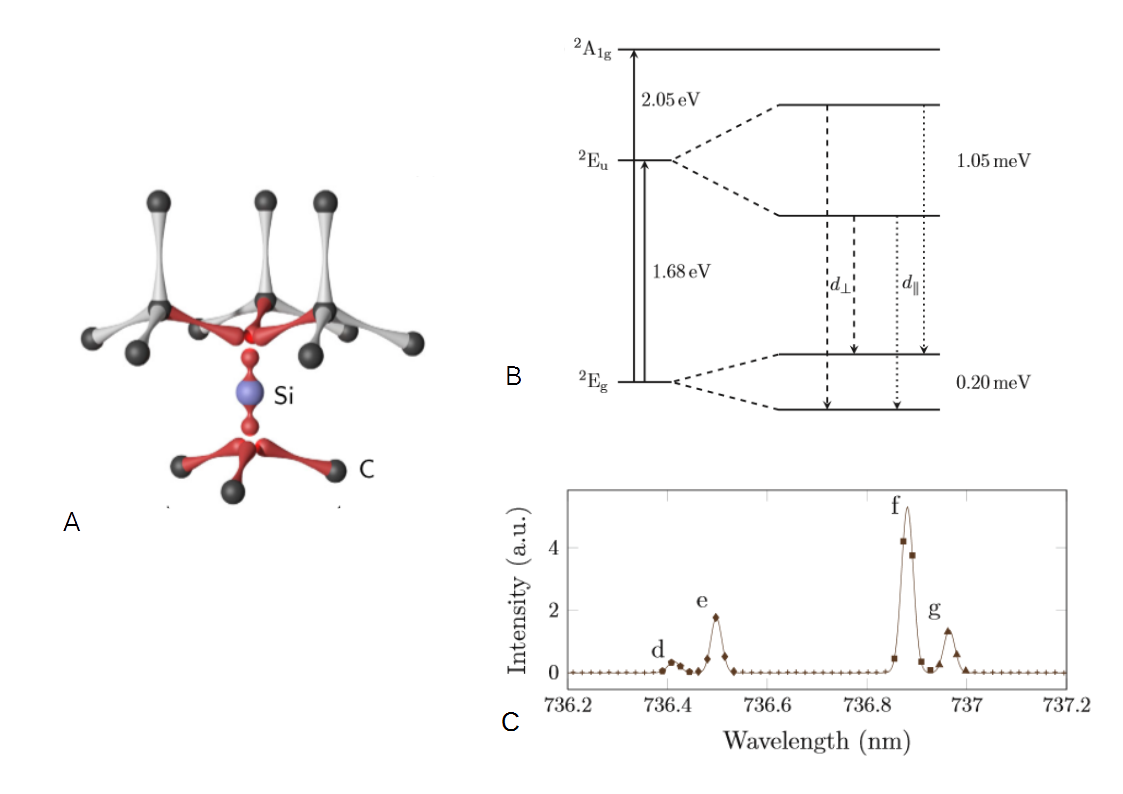
\includegraphics[width=1\linewidth]{Figures/pic/SiV}
\caption{A: SiV center in diamond crystal. B: Four transitions at zero field. C: Corresponding fine structures in ZPL. \citep{ristein_electronic_2000,rogers_all-optical_2014}}
\label{fig:wp20160921204025proli}
\end{figure}

\begin{figure}[h]
\centering
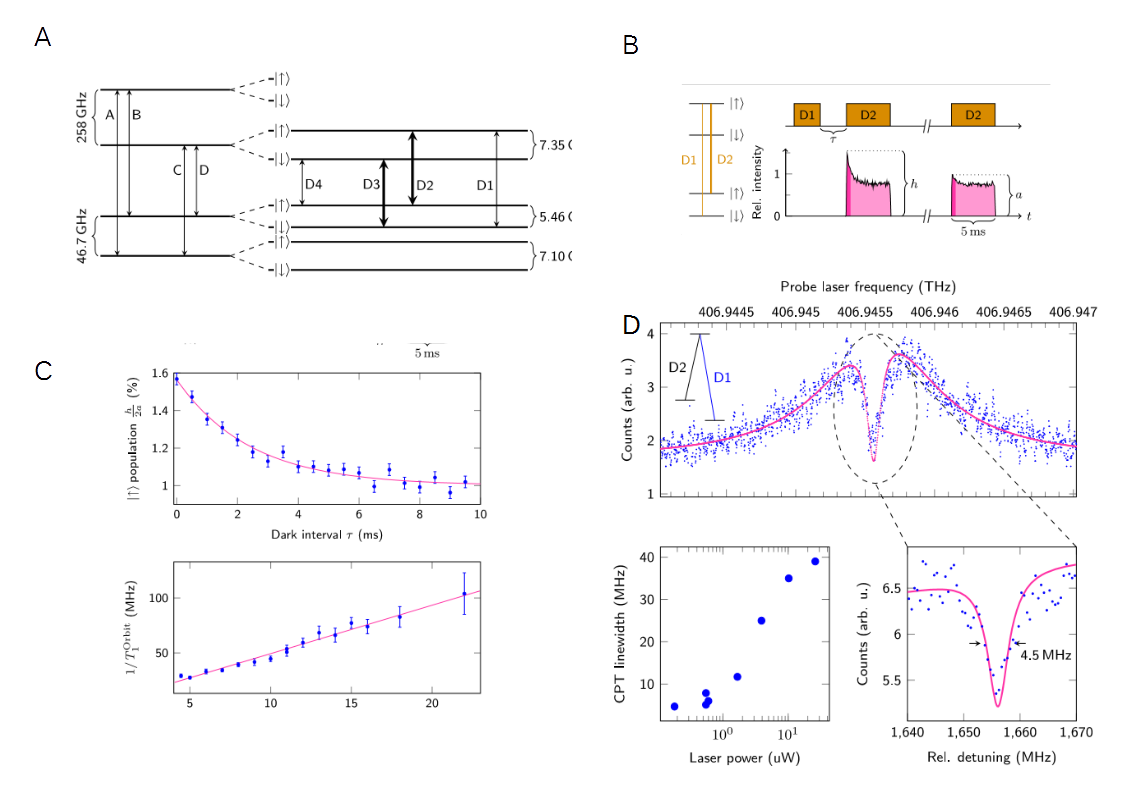
\includegraphics[width=1\linewidth]{Figures/pic/coherent}
\caption{A: Zeeman splitting of the spin=$-\frac{1}{2}$ electronic states. B: A laser pulse resonant to transition D1 flips the spin without producing measurable fluorescence. The initialized spin state can be read out using a laser pulse on the cycling transition D2. C: (Upper) The reduction of h with increasing $\tau$ gives the spin relaxation time at spin $T_{1} = 2.4 \pm 0.2ms$. Interpreting the asymptotic limit a to correspond to thermal spin population suggests a spin initialization fidelity of $h_{\tau=0}/2a = 78\%$. (Lower) Similar pulsed measurements give the orbital relaxation time at 4.5K as orbital $T_{1} = 38\pm1ns$. The orbital relaxation rate $1/T_{1}$ increased linearly with temperature. \citep{rogers_all-optical_2014}}
\label{fig:CPT}
\end{figure}

%----------------------------------------------------------------------------------------

\section[Silicon vacancies in nanodiamonds]{Silicon vacancies in nanodiamonds}
\begin{figure}[h]
\centering
\includegraphics[width=1\linewidth]{Figures/pic/PLEUwe}
\caption{A: Photoluminescence excitation (PLE) spectrum of a single transition with averaged linewidth of 354 MHz. Pink: fit of average. Green: spectral diffusion interpretation. B: Colour map of PLE scan raw data. \citep{jantzen_nanodiamonds_2016}}
\label{fig:PLEUwe}
\end{figure}
As mentioned, one vital problem to solve if we want to use SiV$^{-}$ as a qubit is that, the coherent time has been limited by the rapid orbital relaxation. This is caused by the transition between the degeneracies of ground state which was driven by a single phonon. The elimination of such phonon is an direct approach towards the solution.

The inhibit of orbital relaxation rate can be achieved by the shrinkage of nanodiamond size. Considering the nanodiamond in vacuum as a 3D phonon cavity, a discrete phonon spectrum would be generated. \citep{albrecht_coupling_2013} A particle size smaller than half of the transition phonon length would inhibit the orbital relaxation time. \citep{kleppner_inhibited_1981}

Currently 3 major techniques are employed in the field of nanodiamond fabrication: denotation, chemical vapor deposition (CVD), and high pressure high temperature method (HPHT), while the impurity atoms can be mixed in the beginning or implanted via ion implantation. Since the denotation method produced highly defective diamonds and ion implantation introduces inner strain, for the SiV containing nanodiamonds, HPHT method and CVD method are the top choices.

The principle of the CVD method is to disintegrate the CVD fabricated diamond film, while the HPHT method initializes an phase transition of carbon at high temperature and high pressure. Previously, comparison between the PL spectra of silicon doped polycrystalline diamond films obtained by the CVD method and diamond single crystals grown at a pressure of 6 GPa from a nickel melt at 1500$^{o}C$ has been carried out, and it was demonstrated that the HPHT diamonds exhibit narrower SiV$^{-}$ ZPL lines than CVD fabricated ones \citep{clark_silicon_1995}. HPHT nanodiamonds carrying SiV$^{-}$ with almost lifetime-limited line widths has been reported by Uwe Jantzen \ref{fig:PLEUwe}. \citep{jantzen_nanodiamonds_2016}

%--------------------------------------------------------------------------------------

\section[Motivation of the thesis]{Motivation of the thesis}

The idea of generating longer coherent time via phonon inhibition in nanodiamonds has been put forward, yet not experimentally proved.
\citep{jantzen_nanodiamonds_2016} has reported the narrowest ZPL in nanodiamonds, but the spectral shift/diffusion is a great obstacle preventing people from measuring the orbital relaxation time. 

The mechanism behind the spectral diffusion is yet not clear, but due to the high surface to volume ratio of nanodiamonds, it is highly possible that this phenomenon is connected with the surface conditions. \citep{jantzen_nanodiamonds_2016}

To step further in the research direction of SiV$^{-}$ in nanodiamonds, the current goal is to suppress the spectral diffusion, enabling following measurements (Orbital T1, Spin T1, CPT, etc.) to prove the possibility of acquiring longer coherent time. Since surface treatment has been proved to be capable of manipulating the luminescence of colour centres \citep{stacey_depletion_2012}, it is promising to improve the optical properties of SiV$^{-}$ in nanodiamonds via surface treatment as well. Based on this the experiments in the thesis has been designed.